\documentclass[twoside]{book}

% Packages required by doxygen
\usepackage{fixltx2e}
\usepackage{calc}
\usepackage{doxygen}
\usepackage[export]{adjustbox} % also loads graphicx
\usepackage{graphicx}
\usepackage[utf8]{inputenc}
\usepackage{makeidx}
\usepackage{multicol}
\usepackage{multirow}
\PassOptionsToPackage{warn}{textcomp}
\usepackage{textcomp}
\usepackage[nointegrals]{wasysym}
\usepackage[table]{xcolor}

% Font selection
\usepackage[T1]{fontenc}
\usepackage[scaled=.90]{helvet}
\usepackage{courier}
\usepackage{amssymb}
\usepackage{sectsty}
\renewcommand{\familydefault}{\sfdefault}
\allsectionsfont{%
  \fontseries{bc}\selectfont%
  \color{darkgray}%
}
\renewcommand{\DoxyLabelFont}{%
  \fontseries{bc}\selectfont%
  \color{darkgray}%
}
\newcommand{\+}{\discretionary{\mbox{\scriptsize$\hookleftarrow$}}{}{}}

% Page & text layout
\usepackage{geometry}
\geometry{%
  a4paper,%
  top=2.5cm,%
  bottom=2.5cm,%
  left=2.5cm,%
  right=2.5cm%
}
\tolerance=750
\hfuzz=15pt
\hbadness=750
\setlength{\emergencystretch}{15pt}
\setlength{\parindent}{0cm}
\setlength{\parskip}{3ex plus 2ex minus 2ex}
\makeatletter
\renewcommand{\paragraph}{%
  \@startsection{paragraph}{4}{0ex}{-1.0ex}{1.0ex}{%
    \normalfont\normalsize\bfseries\SS@parafont%
  }%
}
\renewcommand{\subparagraph}{%
  \@startsection{subparagraph}{5}{0ex}{-1.0ex}{1.0ex}{%
    \normalfont\normalsize\bfseries\SS@subparafont%
  }%
}
\makeatother

% Headers & footers
\usepackage{fancyhdr}
\pagestyle{fancyplain}
\fancyhead[LE]{\fancyplain{}{\bfseries\thepage}}
\fancyhead[CE]{\fancyplain{}{}}
\fancyhead[RE]{\fancyplain{}{\bfseries\leftmark}}
\fancyhead[LO]{\fancyplain{}{\bfseries\rightmark}}
\fancyhead[CO]{\fancyplain{}{}}
\fancyhead[RO]{\fancyplain{}{\bfseries\thepage}}
\fancyfoot[LE]{\fancyplain{}{}}
\fancyfoot[CE]{\fancyplain{}{}}
\fancyfoot[RE]{\fancyplain{}{\bfseries\scriptsize Generated by Doxygen }}
\fancyfoot[LO]{\fancyplain{}{\bfseries\scriptsize Generated by Doxygen }}
\fancyfoot[CO]{\fancyplain{}{}}
\fancyfoot[RO]{\fancyplain{}{}}
\renewcommand{\footrulewidth}{0.4pt}
\renewcommand{\chaptermark}[1]{%
  \markboth{#1}{}%
}
\renewcommand{\sectionmark}[1]{%
  \markright{\thesection\ #1}%
}

% Indices & bibliography
\usepackage{natbib}
\usepackage[titles]{tocloft}
\setcounter{tocdepth}{3}
\setcounter{secnumdepth}{5}
\makeindex

% Hyperlinks (required, but should be loaded last)
\usepackage{ifpdf}
\ifpdf
  \usepackage[pdftex,pagebackref=true]{hyperref}
\else
  \usepackage[ps2pdf,pagebackref=true]{hyperref}
\fi
\hypersetup{%
  colorlinks=true,%
  linkcolor=blue,%
  citecolor=blue,%
  unicode%
}

% Custom commands
\newcommand{\clearemptydoublepage}{%
  \newpage{\pagestyle{empty}\cleardoublepage}%
}

\usepackage{caption}
\captionsetup{labelsep=space,justification=centering,font={bf},singlelinecheck=off,skip=4pt,position=top}

%===== C O N T E N T S =====

\begin{document}

% Titlepage & ToC
\hypersetup{pageanchor=false,
             bookmarksnumbered=true,
             pdfencoding=unicode
            }
\pagenumbering{roman}
\begin{titlepage}
\vspace*{7cm}
\begin{center}%
{\Large My Project }\\
\vspace*{1cm}
{\large Generated by Doxygen 1.8.11}\\
\end{center}
\end{titlepage}
\clearemptydoublepage
\tableofcontents
\clearemptydoublepage
\pagenumbering{arabic}
\hypersetup{pageanchor=true}

%--- Begin generated contents ---
\chapter{Namespace Index}
\section{Namespace List}
Here is a list of all namespaces with brief descriptions\+:\begin{DoxyCompactList}
\item\contentsline{section}{\hyperlink{namespacebug__m}{bug\+\_\+m} }{\pageref{namespacebug__m}}{}
\item\contentsline{section}{\hyperlink{namespacego__to__point__service__m}{go\+\_\+to\+\_\+point\+\_\+service\+\_\+m} }{\pageref{namespacego__to__point__service__m}}{}
\item\contentsline{section}{\hyperlink{namespaceuser__interface}{user\+\_\+interface} }{\pageref{namespaceuser__interface}}{}
\item\contentsline{section}{\hyperlink{namespacewall__follow__service__m}{wall\+\_\+follow\+\_\+service\+\_\+m} }{\pageref{namespacewall__follow__service__m}}{}
\end{DoxyCompactList}

\chapter{File Index}
\section{File List}
Here is a list of all files with brief descriptions\+:\begin{DoxyCompactList}
\item\contentsline{section}{scripts/\hyperlink{bug__m_8py}{bug\+\_\+m.\+py} }{\pageref{bug__m_8py}}{}
\item\contentsline{section}{scripts/\hyperlink{go__to__point__service__m_8py}{go\+\_\+to\+\_\+point\+\_\+service\+\_\+m.\+py} }{\pageref{go__to__point__service__m_8py}}{}
\item\contentsline{section}{scripts/\hyperlink{user__interface_8py}{user\+\_\+interface.\+py} }{\pageref{user__interface_8py}}{}
\item\contentsline{section}{scripts/\hyperlink{wall__follow__service__m_8py}{wall\+\_\+follow\+\_\+service\+\_\+m.\+py} }{\pageref{wall__follow__service__m_8py}}{}
\item\contentsline{section}{src/\hyperlink{random__server_8cpp}{random\+\_\+server.\+cpp} }{\pageref{random__server_8cpp}}{}
\item\contentsline{section}{src/\hyperlink{user__interface_8cpp}{user\+\_\+interface.\+cpp} }{\pageref{user__interface_8cpp}}{}
\end{DoxyCompactList}

\chapter{Namespace Documentation}
\hypertarget{namespacebug__m}{}\section{bug\+\_\+m Namespace Reference}
\label{namespacebug__m}\index{bug\+\_\+m@{bug\+\_\+m}}
\subsection*{Functions}
\begin{DoxyCompactItemize}
\item 
def \hyperlink{namespacebug__m_a27cfd2a326148157d3e5e0affbe763f3}{clbk\+\_\+odom} (msg)
\item 
def \hyperlink{namespacebug__m_a6ab3d92b5b6ea12eaa52bf21cfa111f1}{clbk\+\_\+laser} (msg)
\item 
def \hyperlink{namespacebug__m_aca19305feae5c5489e7452e921fcbd9c}{change\+\_\+state} (state)
\item 
def \hyperlink{namespacebug__m_a6547c5ebcd1d3aa3e104a5b573e47862}{normalize\+\_\+angle} (angle)
\item 
def \hyperlink{namespacebug__m_a357589ad533151302b9fa9a893833382}{main} ()
\end{DoxyCompactItemize}
\subsection*{Variables}
\begin{DoxyCompactItemize}
\item 
\hyperlink{namespacebug__m_adc14150838edf40c8028207cd6bb2082}{pub} = None
\item 
\hyperlink{namespacebug__m_abd32bbd25b55f71e56505e72ba56c2f6}{srv\+\_\+client\+\_\+go\+\_\+to\+\_\+point\+\_\+} = None
\item 
\hyperlink{namespacebug__m_af40e8063430e5b54ef2f3f8368338744}{srv\+\_\+client\+\_\+wall\+\_\+follower\+\_\+} = None
\item 
\hyperlink{namespacebug__m_ac6217733c79e361a3bf86e4f51b6ecfd}{srv\+\_\+client\+\_\+user\+\_\+interface\+\_\+} = None
\item 
int \hyperlink{namespacebug__m_a8b5b5c9259592b8efd526c5adb95d95b}{yaw\+\_\+} = 0
\item 
int \hyperlink{namespacebug__m_a23e5e76f14d9d0d139767cb229a53dda}{yaw\+\_\+error\+\_\+allowed\+\_\+} = 5
\item 
\hyperlink{namespacebug__m_ab108d02234aa3ec58605b9f6980ec090}{position\+\_\+} = Point()
\item 
\hyperlink{namespacebug__m_a8fb60e35f164091fe3355d3a0bce95af}{desired\+\_\+position\+\_\+} = Point()
\item 
\hyperlink{namespacebug__m_af10f89c7f929c9babce108f5d7382996}{x}
\item 
\hyperlink{namespacebug__m_ab8596d2ae799585b0d89152b55891aa8}{y}
\item 
\hyperlink{namespacebug__m_afbb54887da57b97920c8d36c6daed1fc}{z}
\item 
\hyperlink{namespacebug__m_ac9d4d95c034fca5a2b5d08ea845bbfcb}{regions\+\_\+} = None
\item 
list \hyperlink{namespacebug__m_ae70f71d3816862f72790fae7bfaa543b}{state\+\_\+desc\+\_\+} = \mbox{[}\textquotesingle{}Go to point\textquotesingle{}, \textquotesingle{}wall following\textquotesingle{}, \textquotesingle{}target reached\textquotesingle{}\mbox{]}
\item 
int \hyperlink{namespacebug__m_a79dc362dff5bef439beacdd5c0c3b2f1}{state\+\_\+} = 0
\end{DoxyCompactItemize}


\subsection{Function Documentation}
\index{bug\+\_\+m@{bug\+\_\+m}!change\+\_\+state@{change\+\_\+state}}
\index{change\+\_\+state@{change\+\_\+state}!bug\+\_\+m@{bug\+\_\+m}}
\subsubsection[{\texorpdfstring{change\+\_\+state(state)}{change_state(state)}}]{\setlength{\rightskip}{0pt plus 5cm}def bug\+\_\+m.\+change\+\_\+state (
\begin{DoxyParamCaption}
\item[{}]{state}
\end{DoxyParamCaption}
)}\hypertarget{namespacebug__m_aca19305feae5c5489e7452e921fcbd9c}{}\label{namespacebug__m_aca19305feae5c5489e7452e921fcbd9c}
\index{bug\+\_\+m@{bug\+\_\+m}!clbk\+\_\+laser@{clbk\+\_\+laser}}
\index{clbk\+\_\+laser@{clbk\+\_\+laser}!bug\+\_\+m@{bug\+\_\+m}}
\subsubsection[{\texorpdfstring{clbk\+\_\+laser(msg)}{clbk_laser(msg)}}]{\setlength{\rightskip}{0pt plus 5cm}def bug\+\_\+m.\+clbk\+\_\+laser (
\begin{DoxyParamCaption}
\item[{}]{msg}
\end{DoxyParamCaption}
)}\hypertarget{namespacebug__m_a6ab3d92b5b6ea12eaa52bf21cfa111f1}{}\label{namespacebug__m_a6ab3d92b5b6ea12eaa52bf21cfa111f1}
\index{bug\+\_\+m@{bug\+\_\+m}!clbk\+\_\+odom@{clbk\+\_\+odom}}
\index{clbk\+\_\+odom@{clbk\+\_\+odom}!bug\+\_\+m@{bug\+\_\+m}}
\subsubsection[{\texorpdfstring{clbk\+\_\+odom(msg)}{clbk_odom(msg)}}]{\setlength{\rightskip}{0pt plus 5cm}def bug\+\_\+m.\+clbk\+\_\+odom (
\begin{DoxyParamCaption}
\item[{}]{msg}
\end{DoxyParamCaption}
)}\hypertarget{namespacebug__m_a27cfd2a326148157d3e5e0affbe763f3}{}\label{namespacebug__m_a27cfd2a326148157d3e5e0affbe763f3}
\index{bug\+\_\+m@{bug\+\_\+m}!main@{main}}
\index{main@{main}!bug\+\_\+m@{bug\+\_\+m}}
\subsubsection[{\texorpdfstring{main()}{main()}}]{\setlength{\rightskip}{0pt plus 5cm}def bug\+\_\+m.\+main (
\begin{DoxyParamCaption}
{}
\end{DoxyParamCaption}
)}\hypertarget{namespacebug__m_a357589ad533151302b9fa9a893833382}{}\label{namespacebug__m_a357589ad533151302b9fa9a893833382}
\index{bug\+\_\+m@{bug\+\_\+m}!normalize\+\_\+angle@{normalize\+\_\+angle}}
\index{normalize\+\_\+angle@{normalize\+\_\+angle}!bug\+\_\+m@{bug\+\_\+m}}
\subsubsection[{\texorpdfstring{normalize\+\_\+angle(angle)}{normalize_angle(angle)}}]{\setlength{\rightskip}{0pt plus 5cm}def bug\+\_\+m.\+normalize\+\_\+angle (
\begin{DoxyParamCaption}
\item[{}]{angle}
\end{DoxyParamCaption}
)}\hypertarget{namespacebug__m_a6547c5ebcd1d3aa3e104a5b573e47862}{}\label{namespacebug__m_a6547c5ebcd1d3aa3e104a5b573e47862}


\subsection{Variable Documentation}
\index{bug\+\_\+m@{bug\+\_\+m}!desired\+\_\+position\+\_\+@{desired\+\_\+position\+\_\+}}
\index{desired\+\_\+position\+\_\+@{desired\+\_\+position\+\_\+}!bug\+\_\+m@{bug\+\_\+m}}
\subsubsection[{\texorpdfstring{desired\+\_\+position\+\_\+}{desired_position_}}]{\setlength{\rightskip}{0pt plus 5cm}bug\+\_\+m.\+desired\+\_\+position\+\_\+ = Point()}\hypertarget{namespacebug__m_a8fb60e35f164091fe3355d3a0bce95af}{}\label{namespacebug__m_a8fb60e35f164091fe3355d3a0bce95af}
\index{bug\+\_\+m@{bug\+\_\+m}!position\+\_\+@{position\+\_\+}}
\index{position\+\_\+@{position\+\_\+}!bug\+\_\+m@{bug\+\_\+m}}
\subsubsection[{\texorpdfstring{position\+\_\+}{position_}}]{\setlength{\rightskip}{0pt plus 5cm}bug\+\_\+m.\+position\+\_\+ = Point()}\hypertarget{namespacebug__m_ab108d02234aa3ec58605b9f6980ec090}{}\label{namespacebug__m_ab108d02234aa3ec58605b9f6980ec090}
\index{bug\+\_\+m@{bug\+\_\+m}!pub@{pub}}
\index{pub@{pub}!bug\+\_\+m@{bug\+\_\+m}}
\subsubsection[{\texorpdfstring{pub}{pub}}]{\setlength{\rightskip}{0pt plus 5cm}bug\+\_\+m.\+pub = None}\hypertarget{namespacebug__m_adc14150838edf40c8028207cd6bb2082}{}\label{namespacebug__m_adc14150838edf40c8028207cd6bb2082}
\index{bug\+\_\+m@{bug\+\_\+m}!regions\+\_\+@{regions\+\_\+}}
\index{regions\+\_\+@{regions\+\_\+}!bug\+\_\+m@{bug\+\_\+m}}
\subsubsection[{\texorpdfstring{regions\+\_\+}{regions_}}]{\setlength{\rightskip}{0pt plus 5cm}bug\+\_\+m.\+regions\+\_\+ = None}\hypertarget{namespacebug__m_ac9d4d95c034fca5a2b5d08ea845bbfcb}{}\label{namespacebug__m_ac9d4d95c034fca5a2b5d08ea845bbfcb}
\index{bug\+\_\+m@{bug\+\_\+m}!srv\+\_\+client\+\_\+go\+\_\+to\+\_\+point\+\_\+@{srv\+\_\+client\+\_\+go\+\_\+to\+\_\+point\+\_\+}}
\index{srv\+\_\+client\+\_\+go\+\_\+to\+\_\+point\+\_\+@{srv\+\_\+client\+\_\+go\+\_\+to\+\_\+point\+\_\+}!bug\+\_\+m@{bug\+\_\+m}}
\subsubsection[{\texorpdfstring{srv\+\_\+client\+\_\+go\+\_\+to\+\_\+point\+\_\+}{srv_client_go_to_point_}}]{\setlength{\rightskip}{0pt plus 5cm}bug\+\_\+m.\+srv\+\_\+client\+\_\+go\+\_\+to\+\_\+point\+\_\+ = None}\hypertarget{namespacebug__m_abd32bbd25b55f71e56505e72ba56c2f6}{}\label{namespacebug__m_abd32bbd25b55f71e56505e72ba56c2f6}
\index{bug\+\_\+m@{bug\+\_\+m}!srv\+\_\+client\+\_\+user\+\_\+interface\+\_\+@{srv\+\_\+client\+\_\+user\+\_\+interface\+\_\+}}
\index{srv\+\_\+client\+\_\+user\+\_\+interface\+\_\+@{srv\+\_\+client\+\_\+user\+\_\+interface\+\_\+}!bug\+\_\+m@{bug\+\_\+m}}
\subsubsection[{\texorpdfstring{srv\+\_\+client\+\_\+user\+\_\+interface\+\_\+}{srv_client_user_interface_}}]{\setlength{\rightskip}{0pt plus 5cm}bug\+\_\+m.\+srv\+\_\+client\+\_\+user\+\_\+interface\+\_\+ = None}\hypertarget{namespacebug__m_ac6217733c79e361a3bf86e4f51b6ecfd}{}\label{namespacebug__m_ac6217733c79e361a3bf86e4f51b6ecfd}
\index{bug\+\_\+m@{bug\+\_\+m}!srv\+\_\+client\+\_\+wall\+\_\+follower\+\_\+@{srv\+\_\+client\+\_\+wall\+\_\+follower\+\_\+}}
\index{srv\+\_\+client\+\_\+wall\+\_\+follower\+\_\+@{srv\+\_\+client\+\_\+wall\+\_\+follower\+\_\+}!bug\+\_\+m@{bug\+\_\+m}}
\subsubsection[{\texorpdfstring{srv\+\_\+client\+\_\+wall\+\_\+follower\+\_\+}{srv_client_wall_follower_}}]{\setlength{\rightskip}{0pt plus 5cm}bug\+\_\+m.\+srv\+\_\+client\+\_\+wall\+\_\+follower\+\_\+ = None}\hypertarget{namespacebug__m_af40e8063430e5b54ef2f3f8368338744}{}\label{namespacebug__m_af40e8063430e5b54ef2f3f8368338744}
\index{bug\+\_\+m@{bug\+\_\+m}!state\+\_\+@{state\+\_\+}}
\index{state\+\_\+@{state\+\_\+}!bug\+\_\+m@{bug\+\_\+m}}
\subsubsection[{\texorpdfstring{state\+\_\+}{state_}}]{\setlength{\rightskip}{0pt plus 5cm}int bug\+\_\+m.\+state\+\_\+ = 0}\hypertarget{namespacebug__m_a79dc362dff5bef439beacdd5c0c3b2f1}{}\label{namespacebug__m_a79dc362dff5bef439beacdd5c0c3b2f1}
\index{bug\+\_\+m@{bug\+\_\+m}!state\+\_\+desc\+\_\+@{state\+\_\+desc\+\_\+}}
\index{state\+\_\+desc\+\_\+@{state\+\_\+desc\+\_\+}!bug\+\_\+m@{bug\+\_\+m}}
\subsubsection[{\texorpdfstring{state\+\_\+desc\+\_\+}{state_desc_}}]{\setlength{\rightskip}{0pt plus 5cm}list bug\+\_\+m.\+state\+\_\+desc\+\_\+ = \mbox{[}\textquotesingle{}Go to point\textquotesingle{}, \textquotesingle{}wall following\textquotesingle{}, \textquotesingle{}target reached\textquotesingle{}\mbox{]}}\hypertarget{namespacebug__m_ae70f71d3816862f72790fae7bfaa543b}{}\label{namespacebug__m_ae70f71d3816862f72790fae7bfaa543b}
\index{bug\+\_\+m@{bug\+\_\+m}!x@{x}}
\index{x@{x}!bug\+\_\+m@{bug\+\_\+m}}
\subsubsection[{\texorpdfstring{x}{x}}]{\setlength{\rightskip}{0pt plus 5cm}bug\+\_\+m.\+x}\hypertarget{namespacebug__m_af10f89c7f929c9babce108f5d7382996}{}\label{namespacebug__m_af10f89c7f929c9babce108f5d7382996}
\index{bug\+\_\+m@{bug\+\_\+m}!y@{y}}
\index{y@{y}!bug\+\_\+m@{bug\+\_\+m}}
\subsubsection[{\texorpdfstring{y}{y}}]{\setlength{\rightskip}{0pt plus 5cm}bug\+\_\+m.\+y}\hypertarget{namespacebug__m_ab8596d2ae799585b0d89152b55891aa8}{}\label{namespacebug__m_ab8596d2ae799585b0d89152b55891aa8}
\index{bug\+\_\+m@{bug\+\_\+m}!yaw\+\_\+@{yaw\+\_\+}}
\index{yaw\+\_\+@{yaw\+\_\+}!bug\+\_\+m@{bug\+\_\+m}}
\subsubsection[{\texorpdfstring{yaw\+\_\+}{yaw_}}]{\setlength{\rightskip}{0pt plus 5cm}int bug\+\_\+m.\+yaw\+\_\+ = 0}\hypertarget{namespacebug__m_a8b5b5c9259592b8efd526c5adb95d95b}{}\label{namespacebug__m_a8b5b5c9259592b8efd526c5adb95d95b}
\index{bug\+\_\+m@{bug\+\_\+m}!yaw\+\_\+error\+\_\+allowed\+\_\+@{yaw\+\_\+error\+\_\+allowed\+\_\+}}
\index{yaw\+\_\+error\+\_\+allowed\+\_\+@{yaw\+\_\+error\+\_\+allowed\+\_\+}!bug\+\_\+m@{bug\+\_\+m}}
\subsubsection[{\texorpdfstring{yaw\+\_\+error\+\_\+allowed\+\_\+}{yaw_error_allowed_}}]{\setlength{\rightskip}{0pt plus 5cm}int bug\+\_\+m.\+yaw\+\_\+error\+\_\+allowed\+\_\+ = 5}\hypertarget{namespacebug__m_a23e5e76f14d9d0d139767cb229a53dda}{}\label{namespacebug__m_a23e5e76f14d9d0d139767cb229a53dda}
\index{bug\+\_\+m@{bug\+\_\+m}!z@{z}}
\index{z@{z}!bug\+\_\+m@{bug\+\_\+m}}
\subsubsection[{\texorpdfstring{z}{z}}]{\setlength{\rightskip}{0pt plus 5cm}bug\+\_\+m.\+z}\hypertarget{namespacebug__m_afbb54887da57b97920c8d36c6daed1fc}{}\label{namespacebug__m_afbb54887da57b97920c8d36c6daed1fc}

\hypertarget{namespacego__to__point__service__m}{}\section{go\+\_\+to\+\_\+point\+\_\+service\+\_\+m Namespace Reference}
\label{namespacego__to__point__service__m}\index{go\+\_\+to\+\_\+point\+\_\+service\+\_\+m@{go\+\_\+to\+\_\+point\+\_\+service\+\_\+m}}
\subsection*{Functions}
\begin{DoxyCompactItemize}
\item 
def \hyperlink{namespacego__to__point__service__m_a5aa5049687ed47c4e5e85903267700ee}{go\+\_\+to\+\_\+point\+\_\+switch} (req)
\item 
def \hyperlink{namespacego__to__point__service__m_a379907ef466483603becace59e6f973b}{clbk\+\_\+odom} (msg)
\item 
def \hyperlink{namespacego__to__point__service__m_a40af22e9a0b3ac0544d0c08b246e6436}{change\+\_\+state} (state)
\item 
def \hyperlink{namespacego__to__point__service__m_a9016b8d25737fe805f75d9db52ff4680}{normalize\+\_\+angle} (angle)
\item 
def \hyperlink{namespacego__to__point__service__m_a45b937484f29d60d6578dd670f07f241}{fix\+\_\+yaw} (des\+\_\+pos)
\item 
def \hyperlink{namespacego__to__point__service__m_aa0efa6e8f30a39de9a6440888882daf1}{go\+\_\+straight\+\_\+ahead} (des\+\_\+pos)
\item 
def \hyperlink{namespacego__to__point__service__m_a22f1876bd87959557a463d43fa521ad3}{done} (des\+\_\+pos)
\item 
def \hyperlink{namespacego__to__point__service__m_a294bca40052b9b1c83ddf85a023b276e}{main} ()
\end{DoxyCompactItemize}
\subsection*{Variables}
\begin{DoxyCompactItemize}
\item 
bool \hyperlink{namespacego__to__point__service__m_a0a0a9847f2d5f0059f48709cba4df15c}{active\+\_\+} = False
\item 
\hyperlink{namespacego__to__point__service__m_abb95705acc8e0b8a82a6fc5d6243bdd8}{position\+\_\+} = Point()
\item 
int \hyperlink{namespacego__to__point__service__m_ab1e499009bca0d4c9ea5e8954aa37797}{yaw\+\_\+} = 0
\item 
int \hyperlink{namespacego__to__point__service__m_a840bab237e425d4f242bf69afe92f767}{state\+\_\+} = 0
\item 
\hyperlink{namespacego__to__point__service__m_a5e4a4244e883c27be9ed897ea5460cc0}{desired\+\_\+position\+\_\+} = Point()
\item 
\hyperlink{namespacego__to__point__service__m_a3ec6e272b02c0f40a625358965caf70b}{x}
\item 
\hyperlink{namespacego__to__point__service__m_a8a0df04be6cfa44113ee26eefbe11f95}{y}
\item 
\hyperlink{namespacego__to__point__service__m_aa0ed9dc81f0153863a2a971384dbcba3}{z}
\item 
int \hyperlink{namespacego__to__point__service__m_af47f1354626111fc63115c06276ae41d}{yaw\+\_\+precision\+\_\+} = math.\+pi/9
\item 
int \hyperlink{namespacego__to__point__service__m_aa642aefafe9c9c963a86f01c5a256e23}{yaw\+\_\+precision\+\_\+2\+\_\+} = math.\+pi/90
\item 
float \hyperlink{namespacego__to__point__service__m_a15a85217148ccc92490d2ec8366dfbd4}{dist\+\_\+precision\+\_\+} = 0.\+3
\item 
float \hyperlink{namespacego__to__point__service__m_a7e9c758884ac92bbb820e532fd32abf6}{kp\+\_\+a} = 3.\+0
\item 
float \hyperlink{namespacego__to__point__service__m_aa9ffa11cdce18c2942bca64db42cb249}{kp\+\_\+d} = 0.\+2
\item 
float \hyperlink{namespacego__to__point__service__m_ac8de1564925338ead12be0a3763b4119}{ub\+\_\+a} = 0.\+6
\item 
float \hyperlink{namespacego__to__point__service__m_a66ab9d35823a86f4fee11da3fa6a7157}{lb\+\_\+a} = -\/0.\+5
\item 
float \hyperlink{namespacego__to__point__service__m_aba661cc0f865736231acaf5b56101b35}{ub\+\_\+d} = 0.\+6
\item 
\hyperlink{namespacego__to__point__service__m_ab9ea0cd28ffda51b5d6f1a436464f861}{pub} = None
\end{DoxyCompactItemize}


\subsection{Function Documentation}
\index{go\+\_\+to\+\_\+point\+\_\+service\+\_\+m@{go\+\_\+to\+\_\+point\+\_\+service\+\_\+m}!change\+\_\+state@{change\+\_\+state}}
\index{change\+\_\+state@{change\+\_\+state}!go\+\_\+to\+\_\+point\+\_\+service\+\_\+m@{go\+\_\+to\+\_\+point\+\_\+service\+\_\+m}}
\subsubsection[{\texorpdfstring{change\+\_\+state(state)}{change_state(state)}}]{\setlength{\rightskip}{0pt plus 5cm}def go\+\_\+to\+\_\+point\+\_\+service\+\_\+m.\+change\+\_\+state (
\begin{DoxyParamCaption}
\item[{}]{state}
\end{DoxyParamCaption}
)}\hypertarget{namespacego__to__point__service__m_a40af22e9a0b3ac0544d0c08b246e6436}{}\label{namespacego__to__point__service__m_a40af22e9a0b3ac0544d0c08b246e6436}
\index{go\+\_\+to\+\_\+point\+\_\+service\+\_\+m@{go\+\_\+to\+\_\+point\+\_\+service\+\_\+m}!clbk\+\_\+odom@{clbk\+\_\+odom}}
\index{clbk\+\_\+odom@{clbk\+\_\+odom}!go\+\_\+to\+\_\+point\+\_\+service\+\_\+m@{go\+\_\+to\+\_\+point\+\_\+service\+\_\+m}}
\subsubsection[{\texorpdfstring{clbk\+\_\+odom(msg)}{clbk_odom(msg)}}]{\setlength{\rightskip}{0pt plus 5cm}def go\+\_\+to\+\_\+point\+\_\+service\+\_\+m.\+clbk\+\_\+odom (
\begin{DoxyParamCaption}
\item[{}]{msg}
\end{DoxyParamCaption}
)}\hypertarget{namespacego__to__point__service__m_a379907ef466483603becace59e6f973b}{}\label{namespacego__to__point__service__m_a379907ef466483603becace59e6f973b}
\index{go\+\_\+to\+\_\+point\+\_\+service\+\_\+m@{go\+\_\+to\+\_\+point\+\_\+service\+\_\+m}!done@{done}}
\index{done@{done}!go\+\_\+to\+\_\+point\+\_\+service\+\_\+m@{go\+\_\+to\+\_\+point\+\_\+service\+\_\+m}}
\subsubsection[{\texorpdfstring{done(des\+\_\+pos)}{done(des_pos)}}]{\setlength{\rightskip}{0pt plus 5cm}def go\+\_\+to\+\_\+point\+\_\+service\+\_\+m.\+done (
\begin{DoxyParamCaption}
\item[{}]{des\+\_\+pos}
\end{DoxyParamCaption}
)}\hypertarget{namespacego__to__point__service__m_a22f1876bd87959557a463d43fa521ad3}{}\label{namespacego__to__point__service__m_a22f1876bd87959557a463d43fa521ad3}
\index{go\+\_\+to\+\_\+point\+\_\+service\+\_\+m@{go\+\_\+to\+\_\+point\+\_\+service\+\_\+m}!fix\+\_\+yaw@{fix\+\_\+yaw}}
\index{fix\+\_\+yaw@{fix\+\_\+yaw}!go\+\_\+to\+\_\+point\+\_\+service\+\_\+m@{go\+\_\+to\+\_\+point\+\_\+service\+\_\+m}}
\subsubsection[{\texorpdfstring{fix\+\_\+yaw(des\+\_\+pos)}{fix_yaw(des_pos)}}]{\setlength{\rightskip}{0pt plus 5cm}def go\+\_\+to\+\_\+point\+\_\+service\+\_\+m.\+fix\+\_\+yaw (
\begin{DoxyParamCaption}
\item[{}]{des\+\_\+pos}
\end{DoxyParamCaption}
)}\hypertarget{namespacego__to__point__service__m_a45b937484f29d60d6578dd670f07f241}{}\label{namespacego__to__point__service__m_a45b937484f29d60d6578dd670f07f241}
\index{go\+\_\+to\+\_\+point\+\_\+service\+\_\+m@{go\+\_\+to\+\_\+point\+\_\+service\+\_\+m}!go\+\_\+straight\+\_\+ahead@{go\+\_\+straight\+\_\+ahead}}
\index{go\+\_\+straight\+\_\+ahead@{go\+\_\+straight\+\_\+ahead}!go\+\_\+to\+\_\+point\+\_\+service\+\_\+m@{go\+\_\+to\+\_\+point\+\_\+service\+\_\+m}}
\subsubsection[{\texorpdfstring{go\+\_\+straight\+\_\+ahead(des\+\_\+pos)}{go_straight_ahead(des_pos)}}]{\setlength{\rightskip}{0pt plus 5cm}def go\+\_\+to\+\_\+point\+\_\+service\+\_\+m.\+go\+\_\+straight\+\_\+ahead (
\begin{DoxyParamCaption}
\item[{}]{des\+\_\+pos}
\end{DoxyParamCaption}
)}\hypertarget{namespacego__to__point__service__m_aa0efa6e8f30a39de9a6440888882daf1}{}\label{namespacego__to__point__service__m_aa0efa6e8f30a39de9a6440888882daf1}
\index{go\+\_\+to\+\_\+point\+\_\+service\+\_\+m@{go\+\_\+to\+\_\+point\+\_\+service\+\_\+m}!go\+\_\+to\+\_\+point\+\_\+switch@{go\+\_\+to\+\_\+point\+\_\+switch}}
\index{go\+\_\+to\+\_\+point\+\_\+switch@{go\+\_\+to\+\_\+point\+\_\+switch}!go\+\_\+to\+\_\+point\+\_\+service\+\_\+m@{go\+\_\+to\+\_\+point\+\_\+service\+\_\+m}}
\subsubsection[{\texorpdfstring{go\+\_\+to\+\_\+point\+\_\+switch(req)}{go_to_point_switch(req)}}]{\setlength{\rightskip}{0pt plus 5cm}def go\+\_\+to\+\_\+point\+\_\+service\+\_\+m.\+go\+\_\+to\+\_\+point\+\_\+switch (
\begin{DoxyParamCaption}
\item[{}]{req}
\end{DoxyParamCaption}
)}\hypertarget{namespacego__to__point__service__m_a5aa5049687ed47c4e5e85903267700ee}{}\label{namespacego__to__point__service__m_a5aa5049687ed47c4e5e85903267700ee}
\index{go\+\_\+to\+\_\+point\+\_\+service\+\_\+m@{go\+\_\+to\+\_\+point\+\_\+service\+\_\+m}!main@{main}}
\index{main@{main}!go\+\_\+to\+\_\+point\+\_\+service\+\_\+m@{go\+\_\+to\+\_\+point\+\_\+service\+\_\+m}}
\subsubsection[{\texorpdfstring{main()}{main()}}]{\setlength{\rightskip}{0pt plus 5cm}def go\+\_\+to\+\_\+point\+\_\+service\+\_\+m.\+main (
\begin{DoxyParamCaption}
{}
\end{DoxyParamCaption}
)}\hypertarget{namespacego__to__point__service__m_a294bca40052b9b1c83ddf85a023b276e}{}\label{namespacego__to__point__service__m_a294bca40052b9b1c83ddf85a023b276e}
\index{go\+\_\+to\+\_\+point\+\_\+service\+\_\+m@{go\+\_\+to\+\_\+point\+\_\+service\+\_\+m}!normalize\+\_\+angle@{normalize\+\_\+angle}}
\index{normalize\+\_\+angle@{normalize\+\_\+angle}!go\+\_\+to\+\_\+point\+\_\+service\+\_\+m@{go\+\_\+to\+\_\+point\+\_\+service\+\_\+m}}
\subsubsection[{\texorpdfstring{normalize\+\_\+angle(angle)}{normalize_angle(angle)}}]{\setlength{\rightskip}{0pt plus 5cm}def go\+\_\+to\+\_\+point\+\_\+service\+\_\+m.\+normalize\+\_\+angle (
\begin{DoxyParamCaption}
\item[{}]{angle}
\end{DoxyParamCaption}
)}\hypertarget{namespacego__to__point__service__m_a9016b8d25737fe805f75d9db52ff4680}{}\label{namespacego__to__point__service__m_a9016b8d25737fe805f75d9db52ff4680}


\subsection{Variable Documentation}
\index{go\+\_\+to\+\_\+point\+\_\+service\+\_\+m@{go\+\_\+to\+\_\+point\+\_\+service\+\_\+m}!active\+\_\+@{active\+\_\+}}
\index{active\+\_\+@{active\+\_\+}!go\+\_\+to\+\_\+point\+\_\+service\+\_\+m@{go\+\_\+to\+\_\+point\+\_\+service\+\_\+m}}
\subsubsection[{\texorpdfstring{active\+\_\+}{active_}}]{\setlength{\rightskip}{0pt plus 5cm}bool go\+\_\+to\+\_\+point\+\_\+service\+\_\+m.\+active\+\_\+ = False}\hypertarget{namespacego__to__point__service__m_a0a0a9847f2d5f0059f48709cba4df15c}{}\label{namespacego__to__point__service__m_a0a0a9847f2d5f0059f48709cba4df15c}
\index{go\+\_\+to\+\_\+point\+\_\+service\+\_\+m@{go\+\_\+to\+\_\+point\+\_\+service\+\_\+m}!desired\+\_\+position\+\_\+@{desired\+\_\+position\+\_\+}}
\index{desired\+\_\+position\+\_\+@{desired\+\_\+position\+\_\+}!go\+\_\+to\+\_\+point\+\_\+service\+\_\+m@{go\+\_\+to\+\_\+point\+\_\+service\+\_\+m}}
\subsubsection[{\texorpdfstring{desired\+\_\+position\+\_\+}{desired_position_}}]{\setlength{\rightskip}{0pt plus 5cm}go\+\_\+to\+\_\+point\+\_\+service\+\_\+m.\+desired\+\_\+position\+\_\+ = Point()}\hypertarget{namespacego__to__point__service__m_a5e4a4244e883c27be9ed897ea5460cc0}{}\label{namespacego__to__point__service__m_a5e4a4244e883c27be9ed897ea5460cc0}
\index{go\+\_\+to\+\_\+point\+\_\+service\+\_\+m@{go\+\_\+to\+\_\+point\+\_\+service\+\_\+m}!dist\+\_\+precision\+\_\+@{dist\+\_\+precision\+\_\+}}
\index{dist\+\_\+precision\+\_\+@{dist\+\_\+precision\+\_\+}!go\+\_\+to\+\_\+point\+\_\+service\+\_\+m@{go\+\_\+to\+\_\+point\+\_\+service\+\_\+m}}
\subsubsection[{\texorpdfstring{dist\+\_\+precision\+\_\+}{dist_precision_}}]{\setlength{\rightskip}{0pt plus 5cm}float go\+\_\+to\+\_\+point\+\_\+service\+\_\+m.\+dist\+\_\+precision\+\_\+ = 0.\+3}\hypertarget{namespacego__to__point__service__m_a15a85217148ccc92490d2ec8366dfbd4}{}\label{namespacego__to__point__service__m_a15a85217148ccc92490d2ec8366dfbd4}
\index{go\+\_\+to\+\_\+point\+\_\+service\+\_\+m@{go\+\_\+to\+\_\+point\+\_\+service\+\_\+m}!kp\+\_\+a@{kp\+\_\+a}}
\index{kp\+\_\+a@{kp\+\_\+a}!go\+\_\+to\+\_\+point\+\_\+service\+\_\+m@{go\+\_\+to\+\_\+point\+\_\+service\+\_\+m}}
\subsubsection[{\texorpdfstring{kp\+\_\+a}{kp_a}}]{\setlength{\rightskip}{0pt plus 5cm}float go\+\_\+to\+\_\+point\+\_\+service\+\_\+m.\+kp\+\_\+a = 3.\+0}\hypertarget{namespacego__to__point__service__m_a7e9c758884ac92bbb820e532fd32abf6}{}\label{namespacego__to__point__service__m_a7e9c758884ac92bbb820e532fd32abf6}
\index{go\+\_\+to\+\_\+point\+\_\+service\+\_\+m@{go\+\_\+to\+\_\+point\+\_\+service\+\_\+m}!kp\+\_\+d@{kp\+\_\+d}}
\index{kp\+\_\+d@{kp\+\_\+d}!go\+\_\+to\+\_\+point\+\_\+service\+\_\+m@{go\+\_\+to\+\_\+point\+\_\+service\+\_\+m}}
\subsubsection[{\texorpdfstring{kp\+\_\+d}{kp_d}}]{\setlength{\rightskip}{0pt plus 5cm}float go\+\_\+to\+\_\+point\+\_\+service\+\_\+m.\+kp\+\_\+d = 0.\+2}\hypertarget{namespacego__to__point__service__m_aa9ffa11cdce18c2942bca64db42cb249}{}\label{namespacego__to__point__service__m_aa9ffa11cdce18c2942bca64db42cb249}
\index{go\+\_\+to\+\_\+point\+\_\+service\+\_\+m@{go\+\_\+to\+\_\+point\+\_\+service\+\_\+m}!lb\+\_\+a@{lb\+\_\+a}}
\index{lb\+\_\+a@{lb\+\_\+a}!go\+\_\+to\+\_\+point\+\_\+service\+\_\+m@{go\+\_\+to\+\_\+point\+\_\+service\+\_\+m}}
\subsubsection[{\texorpdfstring{lb\+\_\+a}{lb_a}}]{\setlength{\rightskip}{0pt plus 5cm}float go\+\_\+to\+\_\+point\+\_\+service\+\_\+m.\+lb\+\_\+a = -\/0.\+5}\hypertarget{namespacego__to__point__service__m_a66ab9d35823a86f4fee11da3fa6a7157}{}\label{namespacego__to__point__service__m_a66ab9d35823a86f4fee11da3fa6a7157}
\index{go\+\_\+to\+\_\+point\+\_\+service\+\_\+m@{go\+\_\+to\+\_\+point\+\_\+service\+\_\+m}!position\+\_\+@{position\+\_\+}}
\index{position\+\_\+@{position\+\_\+}!go\+\_\+to\+\_\+point\+\_\+service\+\_\+m@{go\+\_\+to\+\_\+point\+\_\+service\+\_\+m}}
\subsubsection[{\texorpdfstring{position\+\_\+}{position_}}]{\setlength{\rightskip}{0pt plus 5cm}go\+\_\+to\+\_\+point\+\_\+service\+\_\+m.\+position\+\_\+ = Point()}\hypertarget{namespacego__to__point__service__m_abb95705acc8e0b8a82a6fc5d6243bdd8}{}\label{namespacego__to__point__service__m_abb95705acc8e0b8a82a6fc5d6243bdd8}
\index{go\+\_\+to\+\_\+point\+\_\+service\+\_\+m@{go\+\_\+to\+\_\+point\+\_\+service\+\_\+m}!pub@{pub}}
\index{pub@{pub}!go\+\_\+to\+\_\+point\+\_\+service\+\_\+m@{go\+\_\+to\+\_\+point\+\_\+service\+\_\+m}}
\subsubsection[{\texorpdfstring{pub}{pub}}]{\setlength{\rightskip}{0pt plus 5cm}go\+\_\+to\+\_\+point\+\_\+service\+\_\+m.\+pub = None}\hypertarget{namespacego__to__point__service__m_ab9ea0cd28ffda51b5d6f1a436464f861}{}\label{namespacego__to__point__service__m_ab9ea0cd28ffda51b5d6f1a436464f861}
\index{go\+\_\+to\+\_\+point\+\_\+service\+\_\+m@{go\+\_\+to\+\_\+point\+\_\+service\+\_\+m}!state\+\_\+@{state\+\_\+}}
\index{state\+\_\+@{state\+\_\+}!go\+\_\+to\+\_\+point\+\_\+service\+\_\+m@{go\+\_\+to\+\_\+point\+\_\+service\+\_\+m}}
\subsubsection[{\texorpdfstring{state\+\_\+}{state_}}]{\setlength{\rightskip}{0pt plus 5cm}int go\+\_\+to\+\_\+point\+\_\+service\+\_\+m.\+state\+\_\+ = 0}\hypertarget{namespacego__to__point__service__m_a840bab237e425d4f242bf69afe92f767}{}\label{namespacego__to__point__service__m_a840bab237e425d4f242bf69afe92f767}
\index{go\+\_\+to\+\_\+point\+\_\+service\+\_\+m@{go\+\_\+to\+\_\+point\+\_\+service\+\_\+m}!ub\+\_\+a@{ub\+\_\+a}}
\index{ub\+\_\+a@{ub\+\_\+a}!go\+\_\+to\+\_\+point\+\_\+service\+\_\+m@{go\+\_\+to\+\_\+point\+\_\+service\+\_\+m}}
\subsubsection[{\texorpdfstring{ub\+\_\+a}{ub_a}}]{\setlength{\rightskip}{0pt plus 5cm}float go\+\_\+to\+\_\+point\+\_\+service\+\_\+m.\+ub\+\_\+a = 0.\+6}\hypertarget{namespacego__to__point__service__m_ac8de1564925338ead12be0a3763b4119}{}\label{namespacego__to__point__service__m_ac8de1564925338ead12be0a3763b4119}
\index{go\+\_\+to\+\_\+point\+\_\+service\+\_\+m@{go\+\_\+to\+\_\+point\+\_\+service\+\_\+m}!ub\+\_\+d@{ub\+\_\+d}}
\index{ub\+\_\+d@{ub\+\_\+d}!go\+\_\+to\+\_\+point\+\_\+service\+\_\+m@{go\+\_\+to\+\_\+point\+\_\+service\+\_\+m}}
\subsubsection[{\texorpdfstring{ub\+\_\+d}{ub_d}}]{\setlength{\rightskip}{0pt plus 5cm}float go\+\_\+to\+\_\+point\+\_\+service\+\_\+m.\+ub\+\_\+d = 0.\+6}\hypertarget{namespacego__to__point__service__m_aba661cc0f865736231acaf5b56101b35}{}\label{namespacego__to__point__service__m_aba661cc0f865736231acaf5b56101b35}
\index{go\+\_\+to\+\_\+point\+\_\+service\+\_\+m@{go\+\_\+to\+\_\+point\+\_\+service\+\_\+m}!x@{x}}
\index{x@{x}!go\+\_\+to\+\_\+point\+\_\+service\+\_\+m@{go\+\_\+to\+\_\+point\+\_\+service\+\_\+m}}
\subsubsection[{\texorpdfstring{x}{x}}]{\setlength{\rightskip}{0pt plus 5cm}go\+\_\+to\+\_\+point\+\_\+service\+\_\+m.\+x}\hypertarget{namespacego__to__point__service__m_a3ec6e272b02c0f40a625358965caf70b}{}\label{namespacego__to__point__service__m_a3ec6e272b02c0f40a625358965caf70b}
\index{go\+\_\+to\+\_\+point\+\_\+service\+\_\+m@{go\+\_\+to\+\_\+point\+\_\+service\+\_\+m}!y@{y}}
\index{y@{y}!go\+\_\+to\+\_\+point\+\_\+service\+\_\+m@{go\+\_\+to\+\_\+point\+\_\+service\+\_\+m}}
\subsubsection[{\texorpdfstring{y}{y}}]{\setlength{\rightskip}{0pt plus 5cm}go\+\_\+to\+\_\+point\+\_\+service\+\_\+m.\+y}\hypertarget{namespacego__to__point__service__m_a8a0df04be6cfa44113ee26eefbe11f95}{}\label{namespacego__to__point__service__m_a8a0df04be6cfa44113ee26eefbe11f95}
\index{go\+\_\+to\+\_\+point\+\_\+service\+\_\+m@{go\+\_\+to\+\_\+point\+\_\+service\+\_\+m}!yaw\+\_\+@{yaw\+\_\+}}
\index{yaw\+\_\+@{yaw\+\_\+}!go\+\_\+to\+\_\+point\+\_\+service\+\_\+m@{go\+\_\+to\+\_\+point\+\_\+service\+\_\+m}}
\subsubsection[{\texorpdfstring{yaw\+\_\+}{yaw_}}]{\setlength{\rightskip}{0pt plus 5cm}int go\+\_\+to\+\_\+point\+\_\+service\+\_\+m.\+yaw\+\_\+ = 0}\hypertarget{namespacego__to__point__service__m_ab1e499009bca0d4c9ea5e8954aa37797}{}\label{namespacego__to__point__service__m_ab1e499009bca0d4c9ea5e8954aa37797}
\index{go\+\_\+to\+\_\+point\+\_\+service\+\_\+m@{go\+\_\+to\+\_\+point\+\_\+service\+\_\+m}!yaw\+\_\+precision\+\_\+@{yaw\+\_\+precision\+\_\+}}
\index{yaw\+\_\+precision\+\_\+@{yaw\+\_\+precision\+\_\+}!go\+\_\+to\+\_\+point\+\_\+service\+\_\+m@{go\+\_\+to\+\_\+point\+\_\+service\+\_\+m}}
\subsubsection[{\texorpdfstring{yaw\+\_\+precision\+\_\+}{yaw_precision_}}]{\setlength{\rightskip}{0pt plus 5cm}int go\+\_\+to\+\_\+point\+\_\+service\+\_\+m.\+yaw\+\_\+precision\+\_\+ = math.\+pi/9}\hypertarget{namespacego__to__point__service__m_af47f1354626111fc63115c06276ae41d}{}\label{namespacego__to__point__service__m_af47f1354626111fc63115c06276ae41d}
\index{go\+\_\+to\+\_\+point\+\_\+service\+\_\+m@{go\+\_\+to\+\_\+point\+\_\+service\+\_\+m}!yaw\+\_\+precision\+\_\+2\+\_\+@{yaw\+\_\+precision\+\_\+2\+\_\+}}
\index{yaw\+\_\+precision\+\_\+2\+\_\+@{yaw\+\_\+precision\+\_\+2\+\_\+}!go\+\_\+to\+\_\+point\+\_\+service\+\_\+m@{go\+\_\+to\+\_\+point\+\_\+service\+\_\+m}}
\subsubsection[{\texorpdfstring{yaw\+\_\+precision\+\_\+2\+\_\+}{yaw_precision_2_}}]{\setlength{\rightskip}{0pt plus 5cm}int go\+\_\+to\+\_\+point\+\_\+service\+\_\+m.\+yaw\+\_\+precision\+\_\+2\+\_\+ = math.\+pi/90}\hypertarget{namespacego__to__point__service__m_aa642aefafe9c9c963a86f01c5a256e23}{}\label{namespacego__to__point__service__m_aa642aefafe9c9c963a86f01c5a256e23}
\index{go\+\_\+to\+\_\+point\+\_\+service\+\_\+m@{go\+\_\+to\+\_\+point\+\_\+service\+\_\+m}!z@{z}}
\index{z@{z}!go\+\_\+to\+\_\+point\+\_\+service\+\_\+m@{go\+\_\+to\+\_\+point\+\_\+service\+\_\+m}}
\subsubsection[{\texorpdfstring{z}{z}}]{\setlength{\rightskip}{0pt plus 5cm}go\+\_\+to\+\_\+point\+\_\+service\+\_\+m.\+z}\hypertarget{namespacego__to__point__service__m_aa0ed9dc81f0153863a2a971384dbcba3}{}\label{namespacego__to__point__service__m_aa0ed9dc81f0153863a2a971384dbcba3}

\hypertarget{namespaceuser__interface}{}\section{user\+\_\+interface Namespace Reference}
\label{namespaceuser__interface}\index{user\+\_\+interface@{user\+\_\+interface}}
\subsection*{Functions}
\begin{DoxyCompactItemize}
\item 
def \hyperlink{namespaceuser__interface_aa9dc3b0346ac037400ae347eb6efb788}{set\+\_\+new\+\_\+pos} (req)
\item 
def \hyperlink{namespaceuser__interface_ac26bdb296b6776907b72c17ce5a1b24a}{main} ()
\end{DoxyCompactItemize}


\subsection{Function Documentation}
\index{user\+\_\+interface@{user\+\_\+interface}!main@{main}}
\index{main@{main}!user\+\_\+interface@{user\+\_\+interface}}
\subsubsection[{\texorpdfstring{main()}{main()}}]{\setlength{\rightskip}{0pt plus 5cm}def user\+\_\+interface.\+main (
\begin{DoxyParamCaption}
{}
\end{DoxyParamCaption}
)}\hypertarget{namespaceuser__interface_ac26bdb296b6776907b72c17ce5a1b24a}{}\label{namespaceuser__interface_ac26bdb296b6776907b72c17ce5a1b24a}
\index{user\+\_\+interface@{user\+\_\+interface}!set\+\_\+new\+\_\+pos@{set\+\_\+new\+\_\+pos}}
\index{set\+\_\+new\+\_\+pos@{set\+\_\+new\+\_\+pos}!user\+\_\+interface@{user\+\_\+interface}}
\subsubsection[{\texorpdfstring{set\+\_\+new\+\_\+pos(req)}{set_new_pos(req)}}]{\setlength{\rightskip}{0pt plus 5cm}def user\+\_\+interface.\+set\+\_\+new\+\_\+pos (
\begin{DoxyParamCaption}
\item[{}]{req}
\end{DoxyParamCaption}
)}\hypertarget{namespaceuser__interface_aa9dc3b0346ac037400ae347eb6efb788}{}\label{namespaceuser__interface_aa9dc3b0346ac037400ae347eb6efb788}

\hypertarget{namespacewall__follow__service__m}{}\section{wall\+\_\+follow\+\_\+service\+\_\+m Namespace Reference}
\label{namespacewall__follow__service__m}\index{wall\+\_\+follow\+\_\+service\+\_\+m@{wall\+\_\+follow\+\_\+service\+\_\+m}}
\subsection*{Functions}
\begin{DoxyCompactItemize}
\item 
def \hyperlink{namespacewall__follow__service__m_a8367ccc5f1456166406c0d577d019baf}{wall\+\_\+follower\+\_\+switch} (req)
\item 
def \hyperlink{namespacewall__follow__service__m_ab07be9226f1ee837e03f25d282336b09}{clbk\+\_\+laser} (msg)
\item 
def \hyperlink{namespacewall__follow__service__m_ad99900df1d3fa5dd0683d507b2253b17}{change\+\_\+state} (state)
\item 
def \hyperlink{namespacewall__follow__service__m_a027e1db38933af0544136a5c84de5a83}{take\+\_\+action} ()
\item 
def \hyperlink{namespacewall__follow__service__m_ae65476bf2d8bd9007fda22eaea1ed2b1}{find\+\_\+wall} ()
\item 
def \hyperlink{namespacewall__follow__service__m_aa4262b4e6e90a36c0226c9b90ee97d14}{turn\+\_\+left} ()
\item 
def \hyperlink{namespacewall__follow__service__m_a2f9f1202ed1e75ee80471a9dff56fdbe}{follow\+\_\+the\+\_\+wall} ()
\item 
def \hyperlink{namespacewall__follow__service__m_ab4dbc79e32b45a381737fb7b3c126edf}{main} ()
\end{DoxyCompactItemize}
\subsection*{Variables}
\begin{DoxyCompactItemize}
\item 
bool \hyperlink{namespacewall__follow__service__m_ae80ea3e1537280d2311f2fc113a60bc7}{active\+\_\+} = False
\item 
\hyperlink{namespacewall__follow__service__m_aa66ff19a5a11afad8ec15143f733bea2}{pub\+\_\+} = None
\item 
dictionary \hyperlink{namespacewall__follow__service__m_a30a3b79a68496f06646ee64d67423f36}{regions\+\_\+}
\item 
int \hyperlink{namespacewall__follow__service__m_a1f1e8197a7b86b64c5c2c256173e371d}{state\+\_\+} = 0
\item 
dictionary \hyperlink{namespacewall__follow__service__m_a723d03e512b26cc484d9299418b2773d}{state\+\_\+dict\+\_\+}
\end{DoxyCompactItemize}


\subsection{Function Documentation}
\index{wall\+\_\+follow\+\_\+service\+\_\+m@{wall\+\_\+follow\+\_\+service\+\_\+m}!change\+\_\+state@{change\+\_\+state}}
\index{change\+\_\+state@{change\+\_\+state}!wall\+\_\+follow\+\_\+service\+\_\+m@{wall\+\_\+follow\+\_\+service\+\_\+m}}
\subsubsection[{\texorpdfstring{change\+\_\+state(state)}{change_state(state)}}]{\setlength{\rightskip}{0pt plus 5cm}def wall\+\_\+follow\+\_\+service\+\_\+m.\+change\+\_\+state (
\begin{DoxyParamCaption}
\item[{}]{state}
\end{DoxyParamCaption}
)}\hypertarget{namespacewall__follow__service__m_ad99900df1d3fa5dd0683d507b2253b17}{}\label{namespacewall__follow__service__m_ad99900df1d3fa5dd0683d507b2253b17}
\index{wall\+\_\+follow\+\_\+service\+\_\+m@{wall\+\_\+follow\+\_\+service\+\_\+m}!clbk\+\_\+laser@{clbk\+\_\+laser}}
\index{clbk\+\_\+laser@{clbk\+\_\+laser}!wall\+\_\+follow\+\_\+service\+\_\+m@{wall\+\_\+follow\+\_\+service\+\_\+m}}
\subsubsection[{\texorpdfstring{clbk\+\_\+laser(msg)}{clbk_laser(msg)}}]{\setlength{\rightskip}{0pt plus 5cm}def wall\+\_\+follow\+\_\+service\+\_\+m.\+clbk\+\_\+laser (
\begin{DoxyParamCaption}
\item[{}]{msg}
\end{DoxyParamCaption}
)}\hypertarget{namespacewall__follow__service__m_ab07be9226f1ee837e03f25d282336b09}{}\label{namespacewall__follow__service__m_ab07be9226f1ee837e03f25d282336b09}
\index{wall\+\_\+follow\+\_\+service\+\_\+m@{wall\+\_\+follow\+\_\+service\+\_\+m}!find\+\_\+wall@{find\+\_\+wall}}
\index{find\+\_\+wall@{find\+\_\+wall}!wall\+\_\+follow\+\_\+service\+\_\+m@{wall\+\_\+follow\+\_\+service\+\_\+m}}
\subsubsection[{\texorpdfstring{find\+\_\+wall()}{find_wall()}}]{\setlength{\rightskip}{0pt plus 5cm}def wall\+\_\+follow\+\_\+service\+\_\+m.\+find\+\_\+wall (
\begin{DoxyParamCaption}
{}
\end{DoxyParamCaption}
)}\hypertarget{namespacewall__follow__service__m_ae65476bf2d8bd9007fda22eaea1ed2b1}{}\label{namespacewall__follow__service__m_ae65476bf2d8bd9007fda22eaea1ed2b1}
\index{wall\+\_\+follow\+\_\+service\+\_\+m@{wall\+\_\+follow\+\_\+service\+\_\+m}!follow\+\_\+the\+\_\+wall@{follow\+\_\+the\+\_\+wall}}
\index{follow\+\_\+the\+\_\+wall@{follow\+\_\+the\+\_\+wall}!wall\+\_\+follow\+\_\+service\+\_\+m@{wall\+\_\+follow\+\_\+service\+\_\+m}}
\subsubsection[{\texorpdfstring{follow\+\_\+the\+\_\+wall()}{follow_the_wall()}}]{\setlength{\rightskip}{0pt plus 5cm}def wall\+\_\+follow\+\_\+service\+\_\+m.\+follow\+\_\+the\+\_\+wall (
\begin{DoxyParamCaption}
{}
\end{DoxyParamCaption}
)}\hypertarget{namespacewall__follow__service__m_a2f9f1202ed1e75ee80471a9dff56fdbe}{}\label{namespacewall__follow__service__m_a2f9f1202ed1e75ee80471a9dff56fdbe}
\index{wall\+\_\+follow\+\_\+service\+\_\+m@{wall\+\_\+follow\+\_\+service\+\_\+m}!main@{main}}
\index{main@{main}!wall\+\_\+follow\+\_\+service\+\_\+m@{wall\+\_\+follow\+\_\+service\+\_\+m}}
\subsubsection[{\texorpdfstring{main()}{main()}}]{\setlength{\rightskip}{0pt plus 5cm}def wall\+\_\+follow\+\_\+service\+\_\+m.\+main (
\begin{DoxyParamCaption}
{}
\end{DoxyParamCaption}
)}\hypertarget{namespacewall__follow__service__m_ab4dbc79e32b45a381737fb7b3c126edf}{}\label{namespacewall__follow__service__m_ab4dbc79e32b45a381737fb7b3c126edf}
\index{wall\+\_\+follow\+\_\+service\+\_\+m@{wall\+\_\+follow\+\_\+service\+\_\+m}!take\+\_\+action@{take\+\_\+action}}
\index{take\+\_\+action@{take\+\_\+action}!wall\+\_\+follow\+\_\+service\+\_\+m@{wall\+\_\+follow\+\_\+service\+\_\+m}}
\subsubsection[{\texorpdfstring{take\+\_\+action()}{take_action()}}]{\setlength{\rightskip}{0pt plus 5cm}def wall\+\_\+follow\+\_\+service\+\_\+m.\+take\+\_\+action (
\begin{DoxyParamCaption}
{}
\end{DoxyParamCaption}
)}\hypertarget{namespacewall__follow__service__m_a027e1db38933af0544136a5c84de5a83}{}\label{namespacewall__follow__service__m_a027e1db38933af0544136a5c84de5a83}
\index{wall\+\_\+follow\+\_\+service\+\_\+m@{wall\+\_\+follow\+\_\+service\+\_\+m}!turn\+\_\+left@{turn\+\_\+left}}
\index{turn\+\_\+left@{turn\+\_\+left}!wall\+\_\+follow\+\_\+service\+\_\+m@{wall\+\_\+follow\+\_\+service\+\_\+m}}
\subsubsection[{\texorpdfstring{turn\+\_\+left()}{turn_left()}}]{\setlength{\rightskip}{0pt plus 5cm}def wall\+\_\+follow\+\_\+service\+\_\+m.\+turn\+\_\+left (
\begin{DoxyParamCaption}
{}
\end{DoxyParamCaption}
)}\hypertarget{namespacewall__follow__service__m_aa4262b4e6e90a36c0226c9b90ee97d14}{}\label{namespacewall__follow__service__m_aa4262b4e6e90a36c0226c9b90ee97d14}
\index{wall\+\_\+follow\+\_\+service\+\_\+m@{wall\+\_\+follow\+\_\+service\+\_\+m}!wall\+\_\+follower\+\_\+switch@{wall\+\_\+follower\+\_\+switch}}
\index{wall\+\_\+follower\+\_\+switch@{wall\+\_\+follower\+\_\+switch}!wall\+\_\+follow\+\_\+service\+\_\+m@{wall\+\_\+follow\+\_\+service\+\_\+m}}
\subsubsection[{\texorpdfstring{wall\+\_\+follower\+\_\+switch(req)}{wall_follower_switch(req)}}]{\setlength{\rightskip}{0pt plus 5cm}def wall\+\_\+follow\+\_\+service\+\_\+m.\+wall\+\_\+follower\+\_\+switch (
\begin{DoxyParamCaption}
\item[{}]{req}
\end{DoxyParamCaption}
)}\hypertarget{namespacewall__follow__service__m_a8367ccc5f1456166406c0d577d019baf}{}\label{namespacewall__follow__service__m_a8367ccc5f1456166406c0d577d019baf}


\subsection{Variable Documentation}
\index{wall\+\_\+follow\+\_\+service\+\_\+m@{wall\+\_\+follow\+\_\+service\+\_\+m}!active\+\_\+@{active\+\_\+}}
\index{active\+\_\+@{active\+\_\+}!wall\+\_\+follow\+\_\+service\+\_\+m@{wall\+\_\+follow\+\_\+service\+\_\+m}}
\subsubsection[{\texorpdfstring{active\+\_\+}{active_}}]{\setlength{\rightskip}{0pt plus 5cm}bool wall\+\_\+follow\+\_\+service\+\_\+m.\+active\+\_\+ = False}\hypertarget{namespacewall__follow__service__m_ae80ea3e1537280d2311f2fc113a60bc7}{}\label{namespacewall__follow__service__m_ae80ea3e1537280d2311f2fc113a60bc7}
\index{wall\+\_\+follow\+\_\+service\+\_\+m@{wall\+\_\+follow\+\_\+service\+\_\+m}!pub\+\_\+@{pub\+\_\+}}
\index{pub\+\_\+@{pub\+\_\+}!wall\+\_\+follow\+\_\+service\+\_\+m@{wall\+\_\+follow\+\_\+service\+\_\+m}}
\subsubsection[{\texorpdfstring{pub\+\_\+}{pub_}}]{\setlength{\rightskip}{0pt plus 5cm}wall\+\_\+follow\+\_\+service\+\_\+m.\+pub\+\_\+ = None}\hypertarget{namespacewall__follow__service__m_aa66ff19a5a11afad8ec15143f733bea2}{}\label{namespacewall__follow__service__m_aa66ff19a5a11afad8ec15143f733bea2}
\index{wall\+\_\+follow\+\_\+service\+\_\+m@{wall\+\_\+follow\+\_\+service\+\_\+m}!regions\+\_\+@{regions\+\_\+}}
\index{regions\+\_\+@{regions\+\_\+}!wall\+\_\+follow\+\_\+service\+\_\+m@{wall\+\_\+follow\+\_\+service\+\_\+m}}
\subsubsection[{\texorpdfstring{regions\+\_\+}{regions_}}]{\setlength{\rightskip}{0pt plus 5cm}dictionary wall\+\_\+follow\+\_\+service\+\_\+m.\+regions\+\_\+}\hypertarget{namespacewall__follow__service__m_a30a3b79a68496f06646ee64d67423f36}{}\label{namespacewall__follow__service__m_a30a3b79a68496f06646ee64d67423f36}
{\bfseries Initial value\+:}
\begin{DoxyCode}
1 = \{
2     \textcolor{stringliteral}{'right'}: 0,
3     \textcolor{stringliteral}{'fright'}: 0,
4     \textcolor{stringliteral}{'front'}: 0,
5     \textcolor{stringliteral}{'fleft'}: 0,
6     \textcolor{stringliteral}{'left'}: 0,
7 \}
\end{DoxyCode}
\index{wall\+\_\+follow\+\_\+service\+\_\+m@{wall\+\_\+follow\+\_\+service\+\_\+m}!state\+\_\+@{state\+\_\+}}
\index{state\+\_\+@{state\+\_\+}!wall\+\_\+follow\+\_\+service\+\_\+m@{wall\+\_\+follow\+\_\+service\+\_\+m}}
\subsubsection[{\texorpdfstring{state\+\_\+}{state_}}]{\setlength{\rightskip}{0pt plus 5cm}int wall\+\_\+follow\+\_\+service\+\_\+m.\+state\+\_\+ = 0}\hypertarget{namespacewall__follow__service__m_a1f1e8197a7b86b64c5c2c256173e371d}{}\label{namespacewall__follow__service__m_a1f1e8197a7b86b64c5c2c256173e371d}
\index{wall\+\_\+follow\+\_\+service\+\_\+m@{wall\+\_\+follow\+\_\+service\+\_\+m}!state\+\_\+dict\+\_\+@{state\+\_\+dict\+\_\+}}
\index{state\+\_\+dict\+\_\+@{state\+\_\+dict\+\_\+}!wall\+\_\+follow\+\_\+service\+\_\+m@{wall\+\_\+follow\+\_\+service\+\_\+m}}
\subsubsection[{\texorpdfstring{state\+\_\+dict\+\_\+}{state_dict_}}]{\setlength{\rightskip}{0pt plus 5cm}dictionary wall\+\_\+follow\+\_\+service\+\_\+m.\+state\+\_\+dict\+\_\+}\hypertarget{namespacewall__follow__service__m_a723d03e512b26cc484d9299418b2773d}{}\label{namespacewall__follow__service__m_a723d03e512b26cc484d9299418b2773d}
{\bfseries Initial value\+:}
\begin{DoxyCode}
1 = \{
2     0: \textcolor{stringliteral}{'find the wall'},
3     1: \textcolor{stringliteral}{'turn left'},
4     2: \textcolor{stringliteral}{'follow the wall'},
5 \}
\end{DoxyCode}

\chapter{File Documentation}
\hypertarget{bug__m_8py}{}\section{scripts/bug\+\_\+m.py File Reference}
\label{bug__m_8py}\index{scripts/bug\+\_\+m.\+py@{scripts/bug\+\_\+m.\+py}}
\subsection*{Namespaces}
\begin{DoxyCompactItemize}
\item 
 \hyperlink{namespacebug__m}{bug\+\_\+m}
\end{DoxyCompactItemize}
\subsection*{Functions}
\begin{DoxyCompactItemize}
\item 
def \hyperlink{namespacebug__m_a27cfd2a326148157d3e5e0affbe763f3}{bug\+\_\+m.\+clbk\+\_\+odom} (msg)
\item 
def \hyperlink{namespacebug__m_a6ab3d92b5b6ea12eaa52bf21cfa111f1}{bug\+\_\+m.\+clbk\+\_\+laser} (msg)
\item 
def \hyperlink{namespacebug__m_aca19305feae5c5489e7452e921fcbd9c}{bug\+\_\+m.\+change\+\_\+state} (state)
\item 
def \hyperlink{namespacebug__m_a6547c5ebcd1d3aa3e104a5b573e47862}{bug\+\_\+m.\+normalize\+\_\+angle} (angle)
\item 
def \hyperlink{namespacebug__m_a357589ad533151302b9fa9a893833382}{bug\+\_\+m.\+main} ()
\end{DoxyCompactItemize}
\subsection*{Variables}
\begin{DoxyCompactItemize}
\item 
\hyperlink{namespacebug__m_adc14150838edf40c8028207cd6bb2082}{bug\+\_\+m.\+pub} = None
\item 
\hyperlink{namespacebug__m_abd32bbd25b55f71e56505e72ba56c2f6}{bug\+\_\+m.\+srv\+\_\+client\+\_\+go\+\_\+to\+\_\+point\+\_\+} = None
\item 
\hyperlink{namespacebug__m_af40e8063430e5b54ef2f3f8368338744}{bug\+\_\+m.\+srv\+\_\+client\+\_\+wall\+\_\+follower\+\_\+} = None
\item 
\hyperlink{namespacebug__m_ac6217733c79e361a3bf86e4f51b6ecfd}{bug\+\_\+m.\+srv\+\_\+client\+\_\+user\+\_\+interface\+\_\+} = None
\item 
int \hyperlink{namespacebug__m_a8b5b5c9259592b8efd526c5adb95d95b}{bug\+\_\+m.\+yaw\+\_\+} = 0
\item 
int \hyperlink{namespacebug__m_a23e5e76f14d9d0d139767cb229a53dda}{bug\+\_\+m.\+yaw\+\_\+error\+\_\+allowed\+\_\+} = 5
\item 
\hyperlink{namespacebug__m_ab108d02234aa3ec58605b9f6980ec090}{bug\+\_\+m.\+position\+\_\+} = Point()
\item 
\hyperlink{namespacebug__m_a8fb60e35f164091fe3355d3a0bce95af}{bug\+\_\+m.\+desired\+\_\+position\+\_\+} = Point()
\item 
\hyperlink{namespacebug__m_af10f89c7f929c9babce108f5d7382996}{bug\+\_\+m.\+x}
\item 
\hyperlink{namespacebug__m_ab8596d2ae799585b0d89152b55891aa8}{bug\+\_\+m.\+y}
\item 
\hyperlink{namespacebug__m_afbb54887da57b97920c8d36c6daed1fc}{bug\+\_\+m.\+z}
\item 
\hyperlink{namespacebug__m_ac9d4d95c034fca5a2b5d08ea845bbfcb}{bug\+\_\+m.\+regions\+\_\+} = None
\item 
list \hyperlink{namespacebug__m_ae70f71d3816862f72790fae7bfaa543b}{bug\+\_\+m.\+state\+\_\+desc\+\_\+} = \mbox{[}\textquotesingle{}Go to point\textquotesingle{}, \textquotesingle{}wall following\textquotesingle{}, \textquotesingle{}target reached\textquotesingle{}\mbox{]}
\item 
int \hyperlink{namespacebug__m_a79dc362dff5bef439beacdd5c0c3b2f1}{bug\+\_\+m.\+state\+\_\+} = 0
\end{DoxyCompactItemize}

\hypertarget{go__to__point__service__m_8py}{}\section{scripts/go\+\_\+to\+\_\+point\+\_\+service\+\_\+m.py File Reference}
\label{go__to__point__service__m_8py}\index{scripts/go\+\_\+to\+\_\+point\+\_\+service\+\_\+m.\+py@{scripts/go\+\_\+to\+\_\+point\+\_\+service\+\_\+m.\+py}}
\subsection*{Namespaces}
\begin{DoxyCompactItemize}
\item 
 \hyperlink{namespacego__to__point__service__m}{go\+\_\+to\+\_\+point\+\_\+service\+\_\+m}
\end{DoxyCompactItemize}
\subsection*{Functions}
\begin{DoxyCompactItemize}
\item 
def \hyperlink{namespacego__to__point__service__m_a5aa5049687ed47c4e5e85903267700ee}{go\+\_\+to\+\_\+point\+\_\+service\+\_\+m.\+go\+\_\+to\+\_\+point\+\_\+switch} (req)
\item 
def \hyperlink{namespacego__to__point__service__m_a379907ef466483603becace59e6f973b}{go\+\_\+to\+\_\+point\+\_\+service\+\_\+m.\+clbk\+\_\+odom} (msg)
\item 
def \hyperlink{namespacego__to__point__service__m_a40af22e9a0b3ac0544d0c08b246e6436}{go\+\_\+to\+\_\+point\+\_\+service\+\_\+m.\+change\+\_\+state} (state)
\item 
def \hyperlink{namespacego__to__point__service__m_a9016b8d25737fe805f75d9db52ff4680}{go\+\_\+to\+\_\+point\+\_\+service\+\_\+m.\+normalize\+\_\+angle} (angle)
\item 
def \hyperlink{namespacego__to__point__service__m_a45b937484f29d60d6578dd670f07f241}{go\+\_\+to\+\_\+point\+\_\+service\+\_\+m.\+fix\+\_\+yaw} (des\+\_\+pos)
\item 
def \hyperlink{namespacego__to__point__service__m_aa0efa6e8f30a39de9a6440888882daf1}{go\+\_\+to\+\_\+point\+\_\+service\+\_\+m.\+go\+\_\+straight\+\_\+ahead} (des\+\_\+pos)
\item 
def \hyperlink{namespacego__to__point__service__m_a22f1876bd87959557a463d43fa521ad3}{go\+\_\+to\+\_\+point\+\_\+service\+\_\+m.\+done} (des\+\_\+pos)
\item 
def \hyperlink{namespacego__to__point__service__m_a294bca40052b9b1c83ddf85a023b276e}{go\+\_\+to\+\_\+point\+\_\+service\+\_\+m.\+main} ()
\end{DoxyCompactItemize}
\subsection*{Variables}
\begin{DoxyCompactItemize}
\item 
bool \hyperlink{namespacego__to__point__service__m_a0a0a9847f2d5f0059f48709cba4df15c}{go\+\_\+to\+\_\+point\+\_\+service\+\_\+m.\+active\+\_\+} = False
\item 
\hyperlink{namespacego__to__point__service__m_abb95705acc8e0b8a82a6fc5d6243bdd8}{go\+\_\+to\+\_\+point\+\_\+service\+\_\+m.\+position\+\_\+} = Point()
\item 
int \hyperlink{namespacego__to__point__service__m_ab1e499009bca0d4c9ea5e8954aa37797}{go\+\_\+to\+\_\+point\+\_\+service\+\_\+m.\+yaw\+\_\+} = 0
\item 
int \hyperlink{namespacego__to__point__service__m_a840bab237e425d4f242bf69afe92f767}{go\+\_\+to\+\_\+point\+\_\+service\+\_\+m.\+state\+\_\+} = 0
\item 
\hyperlink{namespacego__to__point__service__m_a5e4a4244e883c27be9ed897ea5460cc0}{go\+\_\+to\+\_\+point\+\_\+service\+\_\+m.\+desired\+\_\+position\+\_\+} = Point()
\item 
\hyperlink{namespacego__to__point__service__m_a3ec6e272b02c0f40a625358965caf70b}{go\+\_\+to\+\_\+point\+\_\+service\+\_\+m.\+x}
\item 
\hyperlink{namespacego__to__point__service__m_a8a0df04be6cfa44113ee26eefbe11f95}{go\+\_\+to\+\_\+point\+\_\+service\+\_\+m.\+y}
\item 
\hyperlink{namespacego__to__point__service__m_aa0ed9dc81f0153863a2a971384dbcba3}{go\+\_\+to\+\_\+point\+\_\+service\+\_\+m.\+z}
\item 
int \hyperlink{namespacego__to__point__service__m_af47f1354626111fc63115c06276ae41d}{go\+\_\+to\+\_\+point\+\_\+service\+\_\+m.\+yaw\+\_\+precision\+\_\+} = math.\+pi/9
\item 
int \hyperlink{namespacego__to__point__service__m_aa642aefafe9c9c963a86f01c5a256e23}{go\+\_\+to\+\_\+point\+\_\+service\+\_\+m.\+yaw\+\_\+precision\+\_\+2\+\_\+} = math.\+pi/90
\item 
float \hyperlink{namespacego__to__point__service__m_a15a85217148ccc92490d2ec8366dfbd4}{go\+\_\+to\+\_\+point\+\_\+service\+\_\+m.\+dist\+\_\+precision\+\_\+} = 0.\+3
\item 
float \hyperlink{namespacego__to__point__service__m_a7e9c758884ac92bbb820e532fd32abf6}{go\+\_\+to\+\_\+point\+\_\+service\+\_\+m.\+kp\+\_\+a} = 3.\+0
\item 
float \hyperlink{namespacego__to__point__service__m_aa9ffa11cdce18c2942bca64db42cb249}{go\+\_\+to\+\_\+point\+\_\+service\+\_\+m.\+kp\+\_\+d} = 0.\+2
\item 
float \hyperlink{namespacego__to__point__service__m_ac8de1564925338ead12be0a3763b4119}{go\+\_\+to\+\_\+point\+\_\+service\+\_\+m.\+ub\+\_\+a} = 0.\+6
\item 
float \hyperlink{namespacego__to__point__service__m_a66ab9d35823a86f4fee11da3fa6a7157}{go\+\_\+to\+\_\+point\+\_\+service\+\_\+m.\+lb\+\_\+a} = -\/0.\+5
\item 
float \hyperlink{namespacego__to__point__service__m_aba661cc0f865736231acaf5b56101b35}{go\+\_\+to\+\_\+point\+\_\+service\+\_\+m.\+ub\+\_\+d} = 0.\+6
\item 
\hyperlink{namespacego__to__point__service__m_ab9ea0cd28ffda51b5d6f1a436464f861}{go\+\_\+to\+\_\+point\+\_\+service\+\_\+m.\+pub} = None
\end{DoxyCompactItemize}

\hypertarget{user__interface_8py}{}\section{scripts/user\+\_\+interface.py File Reference}
\label{user__interface_8py}\index{scripts/user\+\_\+interface.\+py@{scripts/user\+\_\+interface.\+py}}
\subsection*{Namespaces}
\begin{DoxyCompactItemize}
\item 
 \hyperlink{namespaceuser__interface}{user\+\_\+interface}
\end{DoxyCompactItemize}
\subsection*{Functions}
\begin{DoxyCompactItemize}
\item 
def \hyperlink{namespaceuser__interface_aa9dc3b0346ac037400ae347eb6efb788}{user\+\_\+interface.\+set\+\_\+new\+\_\+pos} (req)
\item 
def \hyperlink{namespaceuser__interface_ac26bdb296b6776907b72c17ce5a1b24a}{user\+\_\+interface.\+main} ()
\end{DoxyCompactItemize}

\hypertarget{wall__follow__service__m_8py}{}\section{scripts/wall\+\_\+follow\+\_\+service\+\_\+m.py File Reference}
\label{wall__follow__service__m_8py}\index{scripts/wall\+\_\+follow\+\_\+service\+\_\+m.\+py@{scripts/wall\+\_\+follow\+\_\+service\+\_\+m.\+py}}
\subsection*{Namespaces}
\begin{DoxyCompactItemize}
\item 
 \hyperlink{namespacewall__follow__service__m}{wall\+\_\+follow\+\_\+service\+\_\+m}
\end{DoxyCompactItemize}
\subsection*{Functions}
\begin{DoxyCompactItemize}
\item 
def \hyperlink{namespacewall__follow__service__m_a8367ccc5f1456166406c0d577d019baf}{wall\+\_\+follow\+\_\+service\+\_\+m.\+wall\+\_\+follower\+\_\+switch} (req)
\item 
def \hyperlink{namespacewall__follow__service__m_ab07be9226f1ee837e03f25d282336b09}{wall\+\_\+follow\+\_\+service\+\_\+m.\+clbk\+\_\+laser} (msg)
\item 
def \hyperlink{namespacewall__follow__service__m_ad99900df1d3fa5dd0683d507b2253b17}{wall\+\_\+follow\+\_\+service\+\_\+m.\+change\+\_\+state} (state)
\item 
def \hyperlink{namespacewall__follow__service__m_a027e1db38933af0544136a5c84de5a83}{wall\+\_\+follow\+\_\+service\+\_\+m.\+take\+\_\+action} ()
\item 
def \hyperlink{namespacewall__follow__service__m_ae65476bf2d8bd9007fda22eaea1ed2b1}{wall\+\_\+follow\+\_\+service\+\_\+m.\+find\+\_\+wall} ()
\item 
def \hyperlink{namespacewall__follow__service__m_aa4262b4e6e90a36c0226c9b90ee97d14}{wall\+\_\+follow\+\_\+service\+\_\+m.\+turn\+\_\+left} ()
\item 
def \hyperlink{namespacewall__follow__service__m_a2f9f1202ed1e75ee80471a9dff56fdbe}{wall\+\_\+follow\+\_\+service\+\_\+m.\+follow\+\_\+the\+\_\+wall} ()
\item 
def \hyperlink{namespacewall__follow__service__m_ab4dbc79e32b45a381737fb7b3c126edf}{wall\+\_\+follow\+\_\+service\+\_\+m.\+main} ()
\end{DoxyCompactItemize}
\subsection*{Variables}
\begin{DoxyCompactItemize}
\item 
bool \hyperlink{namespacewall__follow__service__m_ae80ea3e1537280d2311f2fc113a60bc7}{wall\+\_\+follow\+\_\+service\+\_\+m.\+active\+\_\+} = False
\item 
\hyperlink{namespacewall__follow__service__m_aa66ff19a5a11afad8ec15143f733bea2}{wall\+\_\+follow\+\_\+service\+\_\+m.\+pub\+\_\+} = None
\item 
dictionary \hyperlink{namespacewall__follow__service__m_a30a3b79a68496f06646ee64d67423f36}{wall\+\_\+follow\+\_\+service\+\_\+m.\+regions\+\_\+}
\item 
int \hyperlink{namespacewall__follow__service__m_a1f1e8197a7b86b64c5c2c256173e371d}{wall\+\_\+follow\+\_\+service\+\_\+m.\+state\+\_\+} = 0
\item 
dictionary \hyperlink{namespacewall__follow__service__m_a723d03e512b26cc484d9299418b2773d}{wall\+\_\+follow\+\_\+service\+\_\+m.\+state\+\_\+dict\+\_\+}
\end{DoxyCompactItemize}

\hypertarget{random__server_8cpp}{}\section{src/random\+\_\+server.cpp File Reference}
\label{random__server_8cpp}\index{src/random\+\_\+server.\+cpp@{src/random\+\_\+server.\+cpp}}
{\ttfamily \#include \char`\"{}ros/ros.\+h\char`\"{}}\\*
{\ttfamily \#include \char`\"{}final\+\_\+assignment/target.\+h\char`\"{}}\\*
Include dependency graph for random\+\_\+server.\+cpp\+:
\nopagebreak
\begin{figure}[H]
\begin{center}
\leavevmode
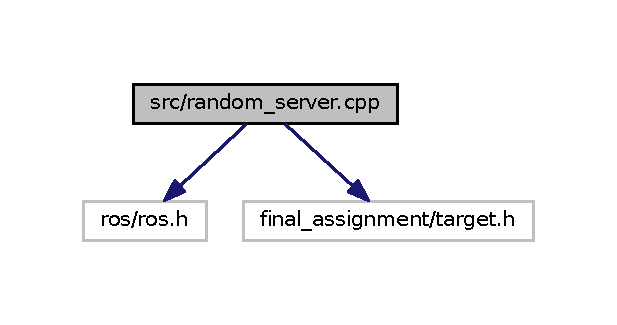
\includegraphics[width=296pt]{random__server_8cpp__incl}
\end{center}
\end{figure}
\subsection*{Functions}
\begin{DoxyCompactItemize}
\item 
int \hyperlink{random__server_8cpp_a44604190463f1e09fb5e63fdf97e9008}{rand\+M\+ToN} (int M, int N)
\item 
bool \hyperlink{random__server_8cpp_ae4fcf433ac117009cf41087a39957c50}{rand\+Target} (final\+\_\+assignment\+::target\+::\+Request \&req, final\+\_\+assignment\+::target\+::\+Response \&res)
\item 
int \hyperlink{random__server_8cpp_a3c04138a5bfe5d72780bb7e82a18e627}{main} (int argc, char $\ast$$\ast$argv)
\end{DoxyCompactItemize}


\subsection{Function Documentation}
\index{random\+\_\+server.\+cpp@{random\+\_\+server.\+cpp}!main@{main}}
\index{main@{main}!random\+\_\+server.\+cpp@{random\+\_\+server.\+cpp}}
\subsubsection[{\texorpdfstring{main(int argc, char $\ast$$\ast$argv)}{main(int argc, char **argv)}}]{\setlength{\rightskip}{0pt plus 5cm}int main (
\begin{DoxyParamCaption}
\item[{int}]{argc, }
\item[{char $\ast$$\ast$}]{argv}
\end{DoxyParamCaption}
)}\hypertarget{random__server_8cpp_a3c04138a5bfe5d72780bb7e82a18e627}{}\label{random__server_8cpp_a3c04138a5bfe5d72780bb7e82a18e627}
\index{random\+\_\+server.\+cpp@{random\+\_\+server.\+cpp}!rand\+M\+ToN@{rand\+M\+ToN}}
\index{rand\+M\+ToN@{rand\+M\+ToN}!random\+\_\+server.\+cpp@{random\+\_\+server.\+cpp}}
\subsubsection[{\texorpdfstring{rand\+M\+To\+N(int M, int N)}{randMToN(int M, int N)}}]{\setlength{\rightskip}{0pt plus 5cm}int rand\+M\+ToN (
\begin{DoxyParamCaption}
\item[{int}]{M, }
\item[{int}]{N}
\end{DoxyParamCaption}
)}\hypertarget{random__server_8cpp_a44604190463f1e09fb5e63fdf97e9008}{}\label{random__server_8cpp_a44604190463f1e09fb5e63fdf97e9008}
\index{random\+\_\+server.\+cpp@{random\+\_\+server.\+cpp}!rand\+Target@{rand\+Target}}
\index{rand\+Target@{rand\+Target}!random\+\_\+server.\+cpp@{random\+\_\+server.\+cpp}}
\subsubsection[{\texorpdfstring{rand\+Target(final\+\_\+assignment\+::target\+::\+Request \&req, final\+\_\+assignment\+::target\+::\+Response \&res)}{randTarget(final_assignment::target::Request &req, final_assignment::target::Response &res)}}]{\setlength{\rightskip}{0pt plus 5cm}bool rand\+Target (
\begin{DoxyParamCaption}
\item[{final\+\_\+assignment\+::target\+::\+Request \&}]{req, }
\item[{final\+\_\+assignment\+::target\+::\+Response \&}]{res}
\end{DoxyParamCaption}
)}\hypertarget{random__server_8cpp_ae4fcf433ac117009cf41087a39957c50}{}\label{random__server_8cpp_ae4fcf433ac117009cf41087a39957c50}

\hypertarget{user__interface_8cpp}{}\section{src/user\+\_\+interface.cpp File Reference}
\label{user__interface_8cpp}\index{src/user\+\_\+interface.\+cpp@{src/user\+\_\+interface.\+cpp}}
{\ttfamily \#include \char`\"{}ros/ros.\+h\char`\"{}}\\*
{\ttfamily \#include \char`\"{}nav\+\_\+msgs/\+Odometry.\+h\char`\"{}}\\*
{\ttfamily \#include \char`\"{}geometry\+\_\+msgs/\+Twist.\+h\char`\"{}}\\*
{\ttfamily \#include \char`\"{}move\+\_\+base\+\_\+msgs/\+Move\+Base\+Action\+Goal.\+h\char`\"{}}\\*
{\ttfamily \#include \char`\"{}final\+\_\+assignment/target.\+h\char`\"{}}\\*
{\ttfamily \#include \char`\"{}std\+\_\+srvs/\+Set\+Bool.\+h\char`\"{}}\\*
Include dependency graph for user\+\_\+interface.\+cpp\+:
\nopagebreak
\begin{figure}[H]
\begin{center}
\leavevmode
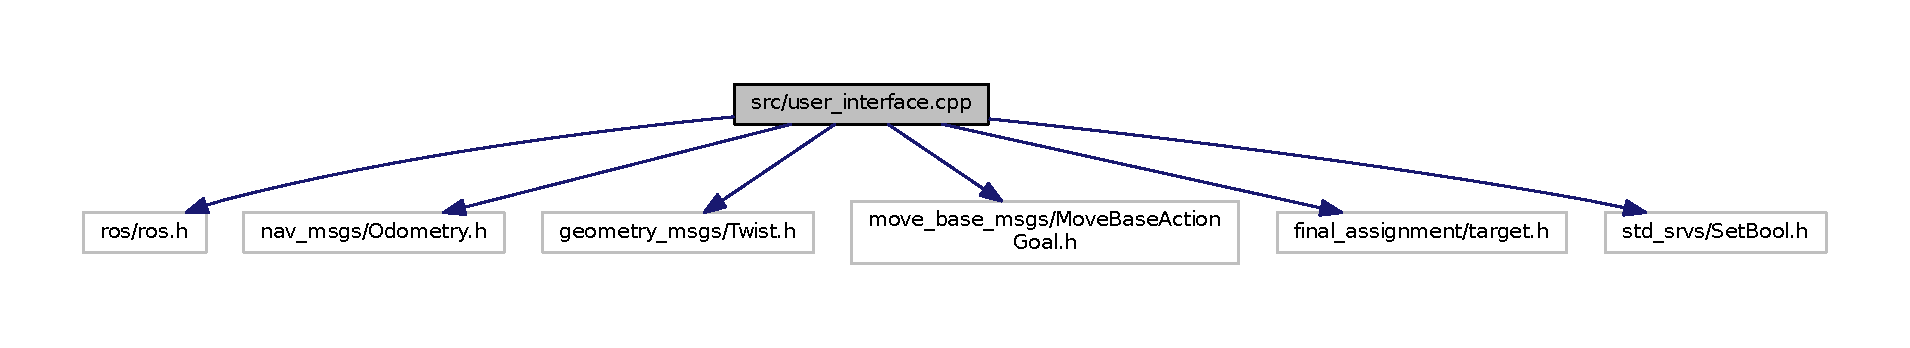
\includegraphics[width=350pt]{user__interface_8cpp__incl}
\end{center}
\end{figure}
\subsection*{Functions}
\begin{DoxyCompactItemize}
\item 
void \hyperlink{user__interface_8cpp_aab6e381bffc34921244a29ec0538ba64}{position\+Callback} (const nav\+\_\+msgs\+::\+Odometry\+::\+Const\+Ptr \&msg)
\item 
int \hyperlink{user__interface_8cpp_a3c04138a5bfe5d72780bb7e82a18e627}{main} (int argc, char $\ast$$\ast$argv)
\end{DoxyCompactItemize}
\subsection*{Variables}
\begin{DoxyCompactItemize}
\item 
ros\+::\+Publisher \hyperlink{user__interface_8cpp_a350594df3e8f6948c8462edfd41ce086}{pub}
\item 
ros\+::\+Subscriber \hyperlink{user__interface_8cpp_a24d694a9a8bf73ee31fe92724886a276}{sub}
\item 
move\+\_\+base\+\_\+msgs\+::\+Move\+Base\+Action\+Goal \hyperlink{user__interface_8cpp_aba8f9ea527086a6bfc77aa9c7f7b695c}{goal\+\_\+pos}
\item 
float \hyperlink{user__interface_8cpp_a51cfe1654cabb04270c9b4bd39a4cd42}{x\+\_\+position}
\item 
float \hyperlink{user__interface_8cpp_a58da4bb03c149b531121f1ab9c7b4e00}{y\+\_\+position}
\item 
final\+\_\+assignment\+::target \hyperlink{user__interface_8cpp_acbca3d0b93cf0ebb255d3191b9c547b0}{random\+\_\+position}
\item 
std\+\_\+srvs\+::\+Set\+Bool \hyperlink{user__interface_8cpp_ae6354788bd23d77103a49beea06f6ed4}{wall\+\_\+follower}
\end{DoxyCompactItemize}


\subsection{Function Documentation}
\index{user\+\_\+interface.\+cpp@{user\+\_\+interface.\+cpp}!main@{main}}
\index{main@{main}!user\+\_\+interface.\+cpp@{user\+\_\+interface.\+cpp}}
\subsubsection[{\texorpdfstring{main(int argc, char $\ast$$\ast$argv)}{main(int argc, char **argv)}}]{\setlength{\rightskip}{0pt plus 5cm}int main (
\begin{DoxyParamCaption}
\item[{int}]{argc, }
\item[{char $\ast$$\ast$}]{argv}
\end{DoxyParamCaption}
)}\hypertarget{user__interface_8cpp_a3c04138a5bfe5d72780bb7e82a18e627}{}\label{user__interface_8cpp_a3c04138a5bfe5d72780bb7e82a18e627}
\index{user\+\_\+interface.\+cpp@{user\+\_\+interface.\+cpp}!position\+Callback@{position\+Callback}}
\index{position\+Callback@{position\+Callback}!user\+\_\+interface.\+cpp@{user\+\_\+interface.\+cpp}}
\subsubsection[{\texorpdfstring{position\+Callback(const nav\+\_\+msgs\+::\+Odometry\+::\+Const\+Ptr \&msg)}{positionCallback(const nav_msgs::Odometry::ConstPtr &msg)}}]{\setlength{\rightskip}{0pt plus 5cm}void position\+Callback (
\begin{DoxyParamCaption}
\item[{const nav\+\_\+msgs\+::\+Odometry\+::\+Const\+Ptr \&}]{msg}
\end{DoxyParamCaption}
)}\hypertarget{user__interface_8cpp_aab6e381bffc34921244a29ec0538ba64}{}\label{user__interface_8cpp_aab6e381bffc34921244a29ec0538ba64}


\subsection{Variable Documentation}
\index{user\+\_\+interface.\+cpp@{user\+\_\+interface.\+cpp}!goal\+\_\+pos@{goal\+\_\+pos}}
\index{goal\+\_\+pos@{goal\+\_\+pos}!user\+\_\+interface.\+cpp@{user\+\_\+interface.\+cpp}}
\subsubsection[{\texorpdfstring{goal\+\_\+pos}{goal_pos}}]{\setlength{\rightskip}{0pt plus 5cm}move\+\_\+base\+\_\+msgs\+::\+Move\+Base\+Action\+Goal goal\+\_\+pos}\hypertarget{user__interface_8cpp_aba8f9ea527086a6bfc77aa9c7f7b695c}{}\label{user__interface_8cpp_aba8f9ea527086a6bfc77aa9c7f7b695c}
\index{user\+\_\+interface.\+cpp@{user\+\_\+interface.\+cpp}!pub@{pub}}
\index{pub@{pub}!user\+\_\+interface.\+cpp@{user\+\_\+interface.\+cpp}}
\subsubsection[{\texorpdfstring{pub}{pub}}]{\setlength{\rightskip}{0pt plus 5cm}ros\+::\+Publisher pub}\hypertarget{user__interface_8cpp_a350594df3e8f6948c8462edfd41ce086}{}\label{user__interface_8cpp_a350594df3e8f6948c8462edfd41ce086}
\index{user\+\_\+interface.\+cpp@{user\+\_\+interface.\+cpp}!random\+\_\+position@{random\+\_\+position}}
\index{random\+\_\+position@{random\+\_\+position}!user\+\_\+interface.\+cpp@{user\+\_\+interface.\+cpp}}
\subsubsection[{\texorpdfstring{random\+\_\+position}{random_position}}]{\setlength{\rightskip}{0pt plus 5cm}final\+\_\+assignment\+::target random\+\_\+position}\hypertarget{user__interface_8cpp_acbca3d0b93cf0ebb255d3191b9c547b0}{}\label{user__interface_8cpp_acbca3d0b93cf0ebb255d3191b9c547b0}
\index{user\+\_\+interface.\+cpp@{user\+\_\+interface.\+cpp}!sub@{sub}}
\index{sub@{sub}!user\+\_\+interface.\+cpp@{user\+\_\+interface.\+cpp}}
\subsubsection[{\texorpdfstring{sub}{sub}}]{\setlength{\rightskip}{0pt plus 5cm}ros\+::\+Subscriber sub}\hypertarget{user__interface_8cpp_a24d694a9a8bf73ee31fe92724886a276}{}\label{user__interface_8cpp_a24d694a9a8bf73ee31fe92724886a276}
\index{user\+\_\+interface.\+cpp@{user\+\_\+interface.\+cpp}!wall\+\_\+follower@{wall\+\_\+follower}}
\index{wall\+\_\+follower@{wall\+\_\+follower}!user\+\_\+interface.\+cpp@{user\+\_\+interface.\+cpp}}
\subsubsection[{\texorpdfstring{wall\+\_\+follower}{wall_follower}}]{\setlength{\rightskip}{0pt plus 5cm}std\+\_\+srvs\+::\+Set\+Bool wall\+\_\+follower}\hypertarget{user__interface_8cpp_ae6354788bd23d77103a49beea06f6ed4}{}\label{user__interface_8cpp_ae6354788bd23d77103a49beea06f6ed4}
\index{user\+\_\+interface.\+cpp@{user\+\_\+interface.\+cpp}!x\+\_\+position@{x\+\_\+position}}
\index{x\+\_\+position@{x\+\_\+position}!user\+\_\+interface.\+cpp@{user\+\_\+interface.\+cpp}}
\subsubsection[{\texorpdfstring{x\+\_\+position}{x_position}}]{\setlength{\rightskip}{0pt plus 5cm}float x\+\_\+position}\hypertarget{user__interface_8cpp_a51cfe1654cabb04270c9b4bd39a4cd42}{}\label{user__interface_8cpp_a51cfe1654cabb04270c9b4bd39a4cd42}
\index{user\+\_\+interface.\+cpp@{user\+\_\+interface.\+cpp}!y\+\_\+position@{y\+\_\+position}}
\index{y\+\_\+position@{y\+\_\+position}!user\+\_\+interface.\+cpp@{user\+\_\+interface.\+cpp}}
\subsubsection[{\texorpdfstring{y\+\_\+position}{y_position}}]{\setlength{\rightskip}{0pt plus 5cm}float y\+\_\+position}\hypertarget{user__interface_8cpp_a58da4bb03c149b531121f1ab9c7b4e00}{}\label{user__interface_8cpp_a58da4bb03c149b531121f1ab9c7b4e00}

%--- End generated contents ---

% Index
\backmatter
\newpage
\phantomsection
\clearemptydoublepage
\addcontentsline{toc}{chapter}{Index}
\printindex

\end{document}
